\chapter{Diseño y análisis} \label{cap:diez}

En este capítulo se describe el análisis del sistema mediante la especificación de casos de uso de los diferentes módulos que lo componen.\\
\newpage

\section{Módulo administrador}
\subsection{Diagrama de casos de uso}

	La figura \ref{fig:moduloAdminCU} muestra los casos de uso del administrador que incluyen la gestión de proyectos y del personal.
	
	\begin{figure}[H]
		\begin{center}
			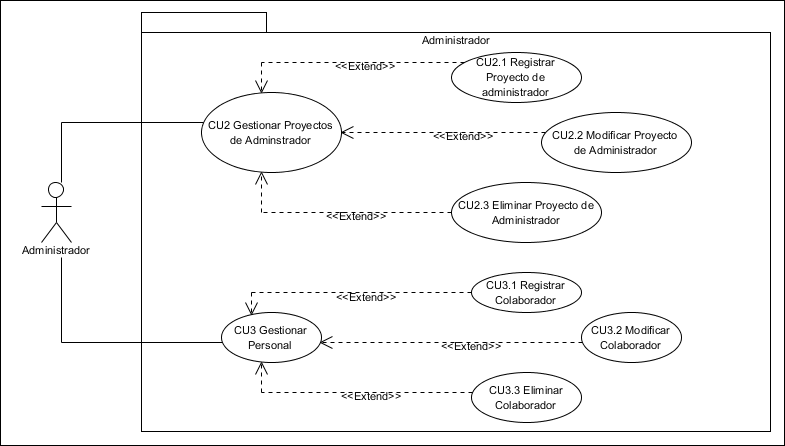
\includegraphics[angle=0,width=.8\textwidth]{images/Diagramas/moduloAdmin}
			\caption{Casos de uso del módulo: Administrador}
			\label{fig:moduloAdminCU}
		\end{center}
	\end{figure}
	\newpage

\subsection{Especificación de los casos de uso}
\subsubsection{Gestión de Colaboradores}
	\input{cu/cu3/CU3}
	\input{cu/cu3/CU3-1}
	\input{cu/cu3/CU3-2}
	\input{cu/cu3/CU3-3}
\subsubsection{Gestión de Proyectos de administrador}
		\begin{UseCase}{CU2}{Gestionar proyectos de Administrador}{
			
		Permite al \hyperlink{admin}{Administrador} realizar las acciones necesarias para controlar los proyectos que han sido previamente registrados en el sistema, como lo son visualizar el listado de los proyectos, registrar un nuevo proyecto, modificarlo o eliminarlo.
		
		La gestión está disponible en cualquier estado en el que se encuentre el proyecto con base en el  \hyperlink{edoProy}{Modelo de estados del proyecto}.
				
	}
		\UCitem{Versión}{\color{Gray}0.1}
		\UCitem{Actor}{\hyperlink{admin}{Administrador}}
		\UCitem{Propósito}{Proporcionar al actor un mecanismo para llevar el control de los proyectos.}
		\UCitem{Entradas}{Ninguna}
		\UCitem{Salidas}{\begin{itemize}
				\item \hyperlink{proyectoEntidad}{Proyecto}: Tabla que muestra la \cdtRef{proyectoEntidad:claveProyecto}{clave}, \cdtRef{proyectoEntidad:nombreProyecto}{nombre} y el \cdtRef{proyectoEntidad:liderProyecto}{Líder de Proyecto} de todos los proyectos existentes.
		\end{itemize}}
		\UCitem{Destino}{Pantalla}
		\UCitem{Precondiciones}{
			\begin{itemize}
				\item Que el usuario haya iniciado sesión como \hyperlink{admin}{Administrador}.
			\end{itemize}	
		}
		\UCitem{Postcondiciones}{Ninguna}
		\UCitem{Errores}{\begin{itemize}
		\item \cdtIdRef{MSG2}{No existe información}: Se muestra en la pantalla \IUref{IU2}{Gestionar proyectos de Administrador} cuando no existen proyectos registrados
		\end{itemize}
		}
		\UCitem{Tipo}{Caso de uso primario}
	\end{UseCase}
%--------------------------------------
	\begin{UCtrayectoria}
		\UCpaso[\UCactor] Solicita gestionar los proyectos presionando la opción ''Proyectos'' del menú \IUref{MN1}{Menú de Administrador}.
		\UCpaso[\UCsist] Obtiene la información de los proyectos registrados en cualquier estado. \hyperlink{CU2:TAA}{[Trayectoria A]}
		\UCpaso[\UCsist] Ordena los proyectos alfabéticamente.
		\UCpaso[\UCsist] Muestra la información de los proyectos en la pantalla \IUref{IU2}{Gestionar proyectos de Administrador}. \label{P3}
		\UCpaso[\UCactor] Gestiona los proyectos a través de los botones: \IUbutton{Registrar}, \editar  y \eliminar. 
	\end{UCtrayectoria}		
%--------------------------------------
	\hypertarget{CU2:TAA}{\textbf{Trayectoria alternativa A}}\\
\noindent \textbf{Condición:} No existen registros de proyectos.
\begin{enumerate}
	\UCpaso[\UCsist] Muestra el mensaje \cdtIdRef{MSG2}{No existe información} en la pantalla \IUref{IU2}{Gestionar proyectos de Administrador} para indicar que no hay registros de proyectos para mostrar.
	\UCpaso[\UCactor] Gestiona los proyectos a través del botón: \IUbutton{Registrar}.
	\item[- -] - - {\em {Fin del caso de uso}}.%
\end{enumerate}
%--------------------------------------

\subsubsection{Puntos de extensión}

\UCExtenssionPoint{El actor requiere registrar un proyecto.}{Paso \ref{P3} de la trayectoria principal.}{\UCref{CU2.1}{Registrar Proyecto}}
\UCExtenssionPoint{El actor requiere modificar un proyecto.}{Paso \ref{P3} de la trayectoria principal.}{\UCref{CU2.2}{Modificar Proyecto}}
\UCExtenssionPoint{El actor requiere eliminar un proyecto.}{Paso \ref{P3} de la trayectoria principal.}{\UCref{CU2.3}{Eliminar Proyecto}}

		\begin{UseCase}{CU2.1}{Registrar proyecto}{
			Permite al {\hyperlink{admin}{Administrador}} registrar la información general de un proyecto en el sistema, dicha información está comprendida por: una \cdtRef{proyectoEntidad:claveProyecto}{clave}, un \cdtRef{proyectoEntidad:nombreProyecto}{nombre} (como medio de identificación), una breve \cdtRef{proyectoEntidad:descripcionProyecto}{descripción} (para definir objetivos y características generales) , la estimación del tiempo que tomará desarrollar el proyecto estableciendo una \cdtRef{proyectoEntidad:fechaIPProyecto}{fecha de inicio programada} y una  \cdtRef{proyectoEntidad:fechaFinPProyecto}{fecha de término programada}, \cdtRef{proyectoEntidad:contraparteProyecto}{contraparte} (en donde se específican los clientes del proyecto o partes interesadas) , el   \cdtRef{proyectoEntidad:presupuestoProyecto}{presupuesto} (en donde se establece el monto calculado del costo del proyecto), el \cdtRef{proyectoEntidad:estadoProyecto}{estado} del proyecto (al momento de registrarlo solo puede ser: En negociación o Iniciado) y por último el \cdtRef{proyectoEntidad:liderProyecto}{líder} (persona encargada de ejecutar las actividades de asociación de colaboradores al proyecto, así como las de terminar, revisar y liberar casos de uso). 
	}
		\UCitem{Versión}{\color{Gray}0.1}
		\UCitem{Actor}{\hyperlink{admin}{Administrador}}
		\UCitem{Propósito}{Registrar la información de un proyecto.}
		\UCitem{Entradas}{
		\begin{itemize}
			\item \cdtRef{proyectoEntidad:claveProyecto}{Clave:} Se escribe desde el teclado.
			\item \cdtRef{proyectoEntidad:nombreProyecto}{Nombre:} Se escribe desde el teclado.
			\item \cdtRef{proyectoEntidad:fechaIProyecto}{Fecha de inicio:} Se selecciona de un calendario.
			\item \cdtRef{proyectoEntidad:fechaFinProyecto}{Fecha de término:} Se selecciona de un calendario.
			\item \cdtRef{proyectoEntidad:fechaIPProyecto}{Fecha de inicio programada:} Se selecciona de un calendario.
			\item \cdtRef{proyectoEntidad:fechaFinPProyecto}{Fecha de término programada:} Se selecciona de un calendario.
			\item \cdtRef{proyectoEntidad:liderProyecto}{Líder del Proyecto:} Se selecciona de una lista.
			\item \cdtRef{proyectoEntidad:descripcionProyecto}{Descripción:} Se escribe desde el teclado.
			\item \cdtRef{proyectoEntidad:contraparteProyecto}{Contraparte} Se escribe desde el teclado.
			\item \cdtRef{proyectoEntidad:presupuestoProyecto}{Presupuesto:} Se escribe desde el teclado.
			\item \hyperlink{tEdoProy}{Estado del Proyecto:} Se selecciona de un lista.
		\end{itemize}	
		}
		\UCitem{Salidas}{\begin{itemize}
				\item \cdtIdRef{MSG1}{Operación exitosa}: Se muestra en la pantalla \IUref{IU2}{Gestionar proyectos de Administrador} para indicar que el registro fue exitoso.
		\end{itemize}}
		\UCitem{Destino}{Pantalla}
		\UCitem{Precondiciones}{
		\begin{itemize}
			\item Interna: Que exista al menos un colaborador registrado.
			\item Interna: Que exista información referente a los estados del proyecto.
		\end{itemize}
		}
		\UCitem{Postcondiciones}{
		\begin{itemize}
			\item Interna: Se registrará un proyecto en el sistema.
			\item Interna: Se podrán gestionar los Términos del glosario, Entidades, Reglas de negocio, Mensajes y Actores.
		\end{itemize}
		}
		\UCitem{Errores}{\begin{itemize}
		\item \cdtIdRef{MSG4}{Dato obligatorio}: Se muestra en la pantalla \IUref{IU2.1}{Registrar proyecto} cuando no se ha ingresado un dato marcado como obligatorio.
		\item \cdtIdRef{MSG29}{Formato incorrecto}: Se muestra en la pantalla \IUref{IU2.1}{Registrar proyecto} cuando el tipo de dato ingresado no cumple con el tipo de dato solicitado en el campo.
		\item \cdtIdRef{MSG6}{Longitud inválida}: Se muestra en la pantalla \IUref{IU2.1}{Registrar proyecto} cuando se ha excedido la longitud de alguno de los campos.
		\item \cdtIdRef{MSG7}{Registro repetido}: Se muestra en la pantalla \IUref{IU2.1}{Registrar proyecto} cuando se registre un proyecto con un nombre o clave que ya se encuentra registrado en el sistema.
		\item \cdtIdRef{MSG12}{Ha ocurrido un error}: Se muestra en la pantalla \IUref{IU2}{Gestionar proyectos de Administrador} cuando no exista información de los estados de un proyecto.
		\item \cdtIdRef{MSG17}{Falta información}: Se muestra en la pantalla \IUref{IU2}{Gestionar proyectos de Administrador} cuando no existan colaboradores registrados.
		\item \cdtIdRef{MSG26}{Orden de fechas}: Se muestra en la pantalla \IUref{IU2.1}{Registrar proyecto} cuando el actor ingrese fechas de término que no son posteriores a las fechas
		de inicio correspondientes.
		\end{itemize}
		}
		\UCitem{Tipo}{Secundario, extiende del caso de uso \UCref{CU2}{Gestionar proyectos de Administrador}.}
	\end{UseCase}
%--------------------------------------
	\begin{UCtrayectoria}
		\UCpaso[\UCactor] Solicita registrar un proyecto oprimiendo el botón \IUbutton{Registrar} de la pantalla \IUref{IU2}{Gestionar proyectos de Administrador}.
		\UCpaso[\UCsist] Verifica que exista información referente a los estados de un proyecto, con base en la regla de negocio \BRref{RN20}{Verificación de catálogos}. \hyperlink{CU2-1:TAA}{[Trayectoria A]}
		\UCpaso[\UCsist] Verifica que exista al menos un colaborador, con base en la regla de negocio \BRref{RN20}{Verificación de catálogos}. \hyperlink{CU2-1:TAB}{[Trayectoria B]}
		\UCpaso[\UCsist] Muestra la pantalla \IUref{IU2.1}{Registrar proyecto}.
		\UCpaso[\UCactor] Ingresa la información solicitada en la pantalla. \label{CU2.1-P5}
		\UCpaso[\UCactor] Solicita guardar el proyecto oprimiendo el botón \IUbutton{Aceptar} de la pantalla \IUref{IU2.1}{Registrar proyecto}. \hyperlink{CU2-1:TAC}{[Trayectoria C]}
		\UCpaso[\UCsist] Verifica que el actor ingrese todos los campos obligatorios con base en la regla de negocio \BRref{RN8}{Datos obligatorios}. \hyperlink{CU2-1:TAD}{[Trayectoria D]}
		\UCpaso[\UCsist] Verificar que los datos ingresados cumpla con la longitud correcta, con base en la regla de negocio \BRref{RN37}{Longitud de datos}. \hyperlink{CU2-1:TAE}{[Trayectoria E]}
		\UCpaso[\UCsist] Verifica que los datos ingresados cumplan con el formato requerido, con base en la regla de negocio \BRref{RN7}{Información correcta}. \hyperlink{CU2-1:TAF}{[Trayectoria F]}
		\UCpaso[\UCsist] Verifica que la clave del proyecto no se encuentre registrada en el sistema con base en la regla de negocio \BRref{RN22}{Unicidad de la clave del Proyecto}. \hyperlink{CU2-1:TAG}{[Trayectoria G]}
		\UCpaso[\UCsist] Verifica que el nombre del proyecto no se encuentre registrado en el sistema con base en la regla de negocio \BRref{RN6}{Unicidad de nombres}. \hyperlink{CU2-1:TAH}{[Trayectoria H]}
		\UCpaso[\UCsist] Verifica que la fecha de término programada sea posterior a la fecha de inicio programada con base en la regla de negocio \BRref{RN35}{Validar Fecha}. \hyperlink{CU2-1:TAI}{[Trayectoria I]}
		\UCpaso[\UCsist] Registra la información del proyecto en el sistema
		\UCpaso[\UCsist] Muestra el mensaje \cdtIdRef{MSG1}{Operación exitosa} en la pantalla \IUref{IU2}{Gestionar proyectos de Administrador} para indicar al actor que el registro se ha realizado exitosamente.
	\end{UCtrayectoria}		
%--------------------------------------
\hypertarget{CU2-1:TAA}{\textbf{Trayectoria alternativa A}}\\
\noindent \textbf{Condición:} El catálogo de estados de un proyecto no tiene información.
\begin{enumerate}
	\UCpaso[\UCsist] Muestra el mensaje \cdtIdRef{MSG16}{Registro Necesario} en la pantalla \IUref{IU2}{Gestionar proyectos de Administrador} para indicar que no es posible realizar la operación debido a la falta de información necesaria para el sistema.
	\item[- -] - - {\em {Fin del caso de uso}}.%
\end{enumerate}

%--------------------------------------
	\hypertarget{CU2-1:TAB}{\textbf{Trayectoria alternativa B}}\\
	\noindent \textbf{Condición:} No hay ningún colaborador registrado.
	\begin{enumerate}
		\UCpaso[\UCsist] Muestra el mensaje \cdtIdRef{MSG16}{Registro necesario} en la pantalla \IUref{IU2}{Gestionar proyectos de Administrador} para indicar que no es posible realizar la operación debido a la falta de información necesaria para el sistema.
		\item[- -] - - {\em {Fin del caso de uso}}.%
	\end{enumerate}
	
%--------------------------------------
\hypertarget{CU2-1:TAC}{\textbf{Trayectoria alternativa C}}\\
\noindent \textbf{Condición:} El actor desea cancelar la operación.
\begin{enumerate}
	\UCpaso[\UCactor] Solicita cancelar la operación oprimiendo el botón \IUbutton{Cancelar} de la pantalla \IUref{IU2.1}{Registrar Proyecto}
	\UCpaso[\UCsist] Muestra la pantalla \IUref{IU2}{Gestionar proyectos de Administrador}.
	\item[- -] - - {\em {Fin del caso de uso}}.%
\end{enumerate}
%--------------------------------------	
\hypertarget{CU2-1:TAD}{\textbf{Trayectoria alternativa D}}\\
\noindent \textbf{Condición:} El actor no ingresó algún dato marcado como obligatorio.
\begin{enumerate}
	\UCpaso[\UCsist] Muestra el mensaje \cdtIdRef{MSG4}{Dato obligatorio} señalando el campo que presenta el error en la pantalla \IUref{IU2.1}{Registrar Proyecto}.
	\UCpaso Regresa al paso \ref{CU2.1-P5} de la trayectoria principal.
	\item[- -] - - {\em {Fin de la trayectoria}}.%
\end{enumerate}
%--------------------------------------
\hypertarget{CU2-1:TAE}{\textbf{Trayectoria alternativa E}}\\
\noindent \textbf{Condición:} El actor ingresó un dato con un número de caracteres fuera del rango permitido.
\begin{enumerate}
	\UCpaso[\UCsist] Muestra el mensaje \cdtIdRef{MSG6}{Longitud inválida} señalando el campo que presenta el error en la pantalla \IUref{IU2.1}{Registrar Proyecto}.
	\UCpaso Regresa al paso \ref{CU2.1-P5} de la trayectoria principal.
	\item[- -] - - {\em {Fin de la trayectoria}}.%
\end{enumerate}
%-------------------------------------
\hypertarget{CU2-1:TAF}{\textbf{Trayectoria alternativa F}}\\
\noindent \textbf{Condición:} El actor ingresó un dato con un formato de dato incorrecto.
\begin{enumerate}
	\UCpaso[\UCsist] Muestra el mensaje \cdtIdRef{MSG29}{Formato incorrecto} señalando el campo que presenta el error en la pantalla \IUref{IU2.1}{Registrar Proyecto}.
	\UCpaso Regresa al paso \ref{CU2.1-P5} de la trayectoria principal.
	\item[- -] - - {\em {Fin de la trayectoria}}.
\end{enumerate}
%--------------------------------------
\hypertarget{CU2-1:TAG}{\textbf{Trayectoria alternativa G}}\\
\noindent \textbf{Condición:} El actor ingresó una clave de proyecto que ya existe dentro del sistema.
\begin{enumerate}
	\UCpaso[\UCsist] Muestra el mensaje \cdtIdRef{MSG7}{Registro repetido} señalando el campo que presenta la duplicidad en la pantalla \IUref{IU2.1}{Registrar Proyecto}.
	\UCpaso Regresa al paso \ref{CU2.1-P5} de la trayectoria principal.
	\item[- -] - - {\em {Fin de la trayectoria}}.
\end{enumerate}
%--------------------------------------	
\hypertarget{CU2-1:TAH}{\textbf{Trayectoria alternativa H}}\\
\noindent \textbf{Condición:} El actor ingresó un nombre de proyecto que ya existe dentro del sistema.
\begin{enumerate}
	\UCpaso[\UCsist] Muestra el mensaje \cdtIdRef{MSG7}{Registro repetido} señalando el campo que presenta la duplicidad en la pantalla \IUref{IU2.1}{Registrar Proyecto}.
	\UCpaso Regresa al paso \ref{CU2.1-P5} de la trayectoria principal.
	\item[- -] - - {\em {Fin de la trayectoria}}.
\end{enumerate}
%--------------------------------------
\hypertarget{CU2-1:TAI}{\textbf{Trayectoria alternativa I}}\\
\noindent \textbf{Condición:} La fecha de termino programada es menor a la fecha de inicio programada.
\begin{enumerate}
	\UCpaso[\UCsist] Muestra el mensaje \cdtIdRef{MSG26}{Orden de fechas} en el campo de fecha de término programada en la pantalla \IUref{IU2.1}{Registrar Proyecto}.
	\UCpaso Regresa al paso \ref{CU2.1-P5} de la trayectoria principal.
	\item[- -] - - {\em {Fin de la trayectoria}}.
\end{enumerate}
\newpage	
\section{Módulo Líder de proyecto}
\subsection{Diagrama de casos de uso}

La figura \ref{fig:moduloLiderA} muestra los casos de uso del líder de análisis que incluyen elegir colaboradores y gestionar proyectos.

\begin{figure}[H]
	\begin{center}
		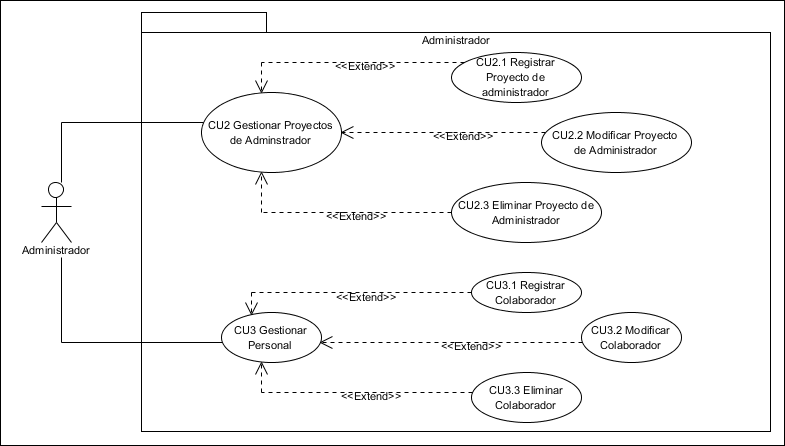
\includegraphics[angle=0,width=.8\textwidth]{images/Diagramas/moduloAdmin}
		\caption{Casos de uso del módulo: Líder de análisis}
		\label{fig:moduloLiderA}
	\end{center}
\end{figure}
\newpage

\subsection{Especificación de los casos de uso}
\subsubsection{Gestión de Proyectos de colaborador}
\input{cu/cu4/CU4}
\input{cu/cu4/CU4-1}
\newpage

\section{Módulo de Módulos}
\subsection{Diagrama de casos de uso}

La figura \ref{fig:moduloLiderM} muestra los casos de uso referentes a la gestión de los módulos.

\begin{figure}[H]
	\begin{center}
		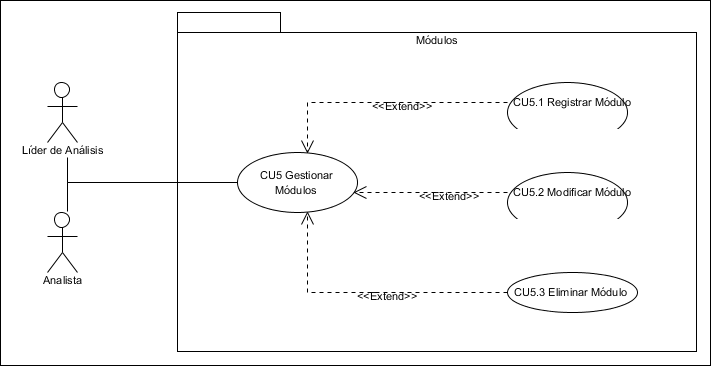
\includegraphics[angle=0,width=.8\textwidth]{images/Diagramas/moduloModulos}
		\caption{Casos de uso del módulo: Módulos}
		\label{fig:moduloLiderM}
	\end{center}
\end{figure}
\newpage

\subsection{Especificación de los casos de uso}
\subsubsection{Gestión de Módulos}
\input{cu/cu5/CU5}
\input{cu/cu5/CU5-1}
\newpage


\section{Módulo de Términos de glosario}
\subsection{Diagrama de casos de uso}

La figura \ref{fig:moduloLiderGLS} muestra los casos de uso referentes a la gestión de los términos de glosario.

\begin{figure}[H]
	\begin{center}
		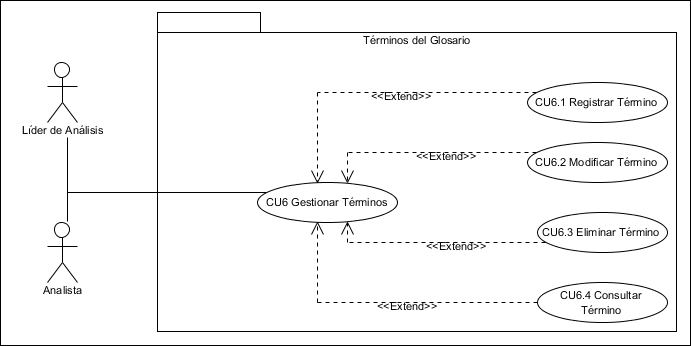
\includegraphics[angle=0,width=.8\textwidth]{images/Diagramas/moduloGLS}
		\caption{Casos de uso del módulo: Términos de Glosario}
		\label{fig:moduloLiderGLS}
	\end{center}
\end{figure}
\newpage

\subsection{Especificación de los casos de uso}
\subsubsection{Gestión de Términos de Glosario}
\input{cu/cu6/CU6}
\input{cu/cu6/CU6-1}
\newpage

\section{Módulo de Entidades y atributos}
\subsection{Diagrama de casos de uso}

La figura \ref{fig:moduloLiderEA} muestra los casos de uso referentes a la gestión de entidades y atributos.

\begin{figure}[H]
	\begin{center}
		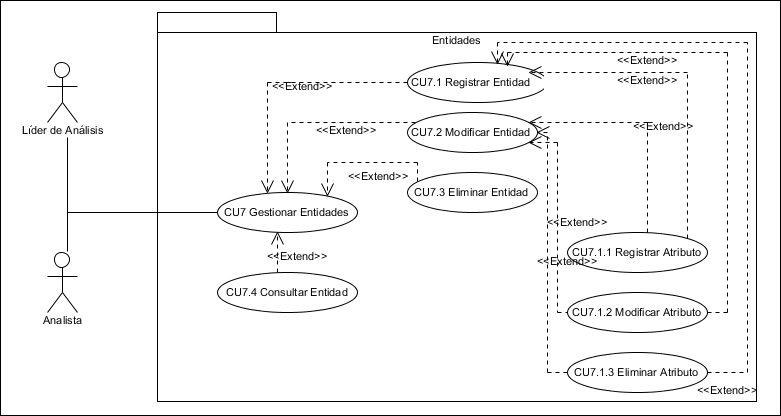
\includegraphics[angle=0,width=.8\textwidth]{images/Diagramas/moduloEntidades}
		\caption{Casos de uso del módulo: Entidades y Atributos}
		\label{fig:moduloLiderEA}
	\end{center}
\end{figure}
\newpage

\subsection{Especificación de los casos de uso}
\subsubsection{Gestión de Entidades}
\input{cu/cu7/CU7}
\input{cu/cu7/CU7-1}
\subsection{Especificación de los casos de uso}
\subsubsection{Gestión de Entidades}
\input{cu/cu7/atributos/CU7-1-1}
\input{cu/cu7/atributos/CU7-1-1-1}
\newpage